% 若编译失败,且生成 .synctex(busy) 辅助文件,可能有两个原因:
% 1. 需要插入的图片不存在:Ctrl + F 搜索 'figure' 将这些代码注释/删除掉即可
% 2. 路径/文件名含中文或空格:更改路径/文件名即可

% --------------------- 文章宏包及相关设置 --------------------- %
% >> ------------------ 文章宏包及相关设置 ------------------ << %
% 设定文章类型与编码格式
\documentclass[UTF8]{article}		

% 物理实验报告所需的其它宏包
\usepackage{ulem}   % \uline 下划线支持
\usepackage{circuitikz} % 电路图 tikz 支持

% 本 .tex 专属的宏定义
    \def\V{\ \mathrm{V}}
    \def\mV{\ \mathrm{mV}}
    \def\kV{\ \mathrm{KV}}
    \def\KV{\ \mathrm{KV}}
    \def\MV{\ \mathrm{MV}}
    \def\A{\ \mathrm{A}}
    \def\mA{\ \mathrm{mA}}
    \def\kA{\ \mathrm{KA}}
    \def\KA{\ \mathrm{KA}}
    \def\MA{\ \mathrm{MA}}
    \def\O{\ \Omega}
    \def\mO{\ \Omega}
    \def\kO{\ \mathrm{K}\Omega}
    \def\KO{\ \mathrm{K}\Omega}
    \def\MO{\ \mathrm{M}\Omega}
    \def\Hz{\ \mathrm{Hz}}

% 自定义宏定义
    \def\N{\mathbb{N}}
    \def\F{\mathbb{F}}
    \def\Z{\mathbb{Z}}
    \def\Q{\mathbb{Q}}
    \def\R{\mathbb{R}}
    \def\C{\mathbb{C}}
    \def\T{\mathbb{T}}
    \def\S{\mathbb{S}}
    %\def\A{\mathbb{A}}
    \def\I{\mathscr{I}}
    \def\d{\mathrm{d}}
    \def\p{\partial}


% 导入基本宏包
    \usepackage[UTF8]{ctex}     % 设置文档为中文语言
    \usepackage{hyperref}  % 宏包:自动生成超链接 (此宏包与标题中的数学环境冲突)
    \hypersetup{
        colorlinks=true,    % false:边框链接 ; true:彩色链接
        citecolor={blue},    % 文献引用颜色
        linkcolor={blue},   % 目录 (我们在目录处单独设置),公式,图表,脚注等内部链接颜色
        urlcolor={orange},    % 网页 URL 链接颜色,包括 \href 中的 text
        % cyan 浅蓝色 
        % magenta 洋红色
        % yellow 黄色
        % black 黑色
        % white 白色
        % red 红色
        % green 绿色
        % blue 蓝色
        % gray 灰色
        % darkgray 深灰色
        % lightgray 浅灰色
        % brown 棕色
        % lime 石灰色
        % olive 橄榄色
        % orange 橙色
        % pink 粉红色
        % purple 紫色
        % teal 蓝绿色
        % violet 紫罗兰色
    }
    % \usepackage{docmute}    % 宏包:子文件导入时自动去除导言区,用于主/子文件的写作方式,\include{./51单片机笔记}即可。注:启用此宏包会导致.tex文件capacity受限。
    \usepackage{amsmath}    % 宏包:数学公式
    \usepackage{mathrsfs}   % 宏包:提供更多数学符号
    \usepackage{amssymb}    % 宏包:提供更多数学符号
    \usepackage{pifont}     % 宏包:提供了特殊符号和字体
    \usepackage{extarrows}  % 宏包:更多箭头符号 
    \usepackage{multicol}   % 宏包:支持多栏 

% 文章页面margin设置
    \usepackage[a4paper]{geometry}
        \geometry{top=0.75in}
        \geometry{bottom=0.75in}
        \geometry{left=0.75in}
        \geometry{right=0.75in}   % 设置上下左右页边距
        \geometry{marginparwidth=1.75cm}    % 设置边注距离(注释、标记等)

% 配置数学环境
    \usepackage{amsthm} % 宏包:数学环境配置
    % theorem-line 环境自定义
        \newtheoremstyle{MyLineTheoremStyle}% <name>
            {11pt}% <space above>
            {11pt}% <space below>
            {\kaishu}% <body font> 默认使用正文字体, \kaishu 为楷体
            {}% <indent amount>
            {\bfseries}% <theorem head font> 设置标题项为加粗
            {:\ \ }% <punctuation after theorem head>
            {.5em}% <space after theorem head>
            {\textbf{#1}\thmnumber{#2}\ \ (\,\textbf{#3}\,)}% 设置标题内容顺序
        \theoremstyle{MyLineTheoremStyle} % 应用自定义的定理样式
        \newtheorem{LineTheorem}{Theorem.\,}
    % theorem-block 环境自定义
        \newtheoremstyle{MyBlockTheoremStyle}% <name>
            {11pt}% <space above>
            {11pt}% <space below>
            {\kaishu}% <body font> 使用默认正文字体
            {}% <indent amount>
            {\bfseries}% <theorem head font> 设置标题项为加粗
            {:\\ \indent}% <punctuation after theorem head>
            {.5em}% <space after theorem head>
            {\textbf{#1}\thmnumber{#2}\ \ (\,\textbf{#3}\,)}% 设置标题内容顺序
        \theoremstyle{MyBlockTheoremStyle} % 应用自定义的定理样式
        \newtheorem{BlockTheorem}[LineTheorem]{Theorem.\,} % 使用 LineTheorem 的计数器
    % definition 环境自定义
        \newtheoremstyle{MySubsubsectionStyle}% <name>
            {11pt}% <space above>
            {11pt}% <space below>
            {}% <body font> 使用默认正文字体
            {}% <indent amount>
            {\bfseries}% <theorem head font> 设置标题项为加粗
            {\\ \indent}% <punctuation after theorem head>
            {0pt}% <space after theorem head>
            {\textbf{#3}}% 设置标题内容顺序
        \theoremstyle{MySubsubsectionStyle} % 应用自定义的定理样式
        \newtheorem{definition}{}

%宏包:有色文本框(proof环境)及其设置
    \usepackage{xcolor}    %设置插入的文本框颜色
    \usepackage[strict]{changepage}     % 提供一个 adjustwidth 环境
    \usepackage{framed}     % 实现方框效果
        \definecolor{graybox_color}{rgb}{0.95,0.95,0.96} % 文本框颜色。修改此行中的 rgb 数值即可改变方框纹颜色,具体颜色的rgb数值可以在网站https://colordrop.io/ 中获得。(截止目前的尝试还没有成功过,感觉单位不一样)(找到喜欢的颜色,点击下方的小眼睛,找到rgb值,复制修改即可)
        \newenvironment{graybox}{%
        \def\FrameCommand{%
        \hspace{1pt}%
        {\color{gray}\small \vrule width 2pt}%
        {\color{graybox_color}\vrule width 4pt}%
        \colorbox{graybox_color}%
        }%
        \MakeFramed{\advance\hsize-\width\FrameRestore}%
        \noindent\hspace{-4.55pt}% disable indenting first paragraph
        \begin{adjustwidth}{}{7pt}%
        \vspace{2pt}\vspace{2pt}%
        }
        {%
        \vspace{2pt}\end{adjustwidth}\endMakeFramed%
        }

% 外源代码插入设置
    % matlab 代码插入设置
    \usepackage{matlab-prettifier}
        \lstset{style=Matlab-editor}    % 继承 matlab 代码高亮 , 此行不能删去
    \usepackage[most]{tcolorbox} % 引入tcolorbox包 
    \usepackage{listings} % 引入listings包
        \tcbuselibrary{listings, skins, breakable}
        \newfontfamily\codefont{Consolas} % 定义需要的 codefont 字体
        \lstdefinestyle{MatlabStyle_inc}{   % 插入代码的样式
            language=Matlab,
            basicstyle=\small\ttfamily\codefont,    % ttfamily 确保等宽 
            breakatwhitespace=false,
            breaklines=true,
            captionpos=b,
            keepspaces=true,
            numbers=left,
            numbersep=15pt,
            showspaces=false,
            showstringspaces=false,
            showtabs=false,
            tabsize=2,
            xleftmargin=15pt,   % 左边距
            %frame=single, % single 为包围式单线框
            frame=shadowbox,    % shadowbox 为带阴影包围式单线框效果
            %escapeinside=``,   % 允许在代码块中使用 LaTeX 命令 (此行无用)
            %frameround=tttt,    % tttt 表示四个角都是圆角
            framextopmargin=0pt,    % 边框上边距
            framexbottommargin=0pt, % 边框下边距
            framexleftmargin=5pt,   % 边框左边距
            framexrightmargin=5pt,  % 边框右边距
            rulesepcolor=\color{red!20!green!20!blue!20}, % 阴影框颜色设置
            %backgroundcolor=\color{blue!10}, % 背景颜色
        }
        \lstdefinestyle{MatlabStyle_src}{   % 插入代码的样式
            language=Matlab,
            basicstyle=\small\ttfamily\codefont,    % ttfamily 确保等宽 
            breakatwhitespace=false,
            breaklines=true,
            captionpos=b,
            keepspaces=true,
            numbers=left,
            numbersep=15pt,
            showspaces=false,
            showstringspaces=false,
            showtabs=false,
            tabsize=2,
        }
        \newtcblisting{matlablisting}{
            %arc=2pt,        % 圆角半径
            % 调整代码在 listing 中的位置以和引入文件时的格式相同
            top=0pt,
            bottom=0pt,
            left=-5pt,
            right=-5pt,
            listing only,   % 此句不能删去
            listing style=MatlabStyle_src,
            breakable,
            colback=white,   % 选一个合适的颜色
            colframe=black!0,   % 感叹号后跟不透明度 (为 0 时完全透明)
        }
        \lstset{
            style=MatlabStyle_inc,
        }

% table 支持
    \usepackage{booktabs}   % 宏包:三线表
    \usepackage{tabularray} % 宏包:表格排版
    \usepackage{longtable}  % 宏包:长表格
    \usepackage{diagbox}    % 宏包:对角线表头

% figure 设置
    \usepackage{graphicx}  % 支持 jpg, png, eps, pdf 图片 
    \usepackage{svg}       % 支持 svg 图片
        \svgsetup{
            % 指向 inkscape.exe 的路径
            inkscapeexe = C:/aa_MySame/inkscape/bin/inkscape.exe, 
            % 一定程度上修复导入后图片文字溢出几何图形的问题
            inkscapelatex = false                 
        }
    \usepackage{subcaption} % 用于子图和小图注  

% 图表进阶设置
    \usepackage{caption}    % 图注、表注
        \captionsetup[figure]{name=图}  
        \captionsetup[table]{name=表}
        \captionsetup{
            labelfont=bf, % 设置标签为粗体
            textfont=bf,  % 设置文本为粗体
            font=small  
        }
    \usepackage{float}     % 图表位置浮动设置 

% 圆圈序号自定义
    \newcommand*\circled[1]{\tikz[baseline=(char.base)]{\node[shape=circle,draw,inner sep=0.8pt, line width = 0.03em] (char) {\small \bfseries #1};}}   % TikZ solution

% 列表设置
    \usepackage{enumitem}   % 宏包:列表环境设置
        \setlist[enumerate]{
            label=(\arabic*) ,   % 设置序号样式为加粗的 (1) (2) (3)
            ref=\arabic*, % 如果需要引用列表项,这将决定引用格式(这里仍然使用数字)
            itemsep=0pt, parsep=0pt, topsep=0pt, partopsep=0pt, leftmargin=3.5em} 
        \setlist[itemize]{itemsep=0pt, parsep=0pt, topsep=0pt, partopsep=0pt, leftmargin=3.5em}
        \newlist{circledenum}{enumerate}{1} % 创建一个新的枚举环境  
        \setlist[circledenum,1]{  
            label=\protect\circled{\arabic*}, % 使用 \arabic* 来获取当前枚举计数器的值,并用 \circled 包装它  
            ref=\arabic*, % 如果需要引用列表项,这将决定引用格式(这里仍然使用数字)
            itemsep=0pt, parsep=0pt, topsep=0pt, partopsep=0pt, leftmargin=3.5em
        }  

% 其它设置
    % 脚注设置
        \renewcommand\thefootnote{\ding{\numexpr171+\value{footnote}}}
    % 参考文献引用设置
        \bibliographystyle{unsrt}   % 设置参考文献引用格式为unsrt
        \newcommand{\upcite}[1]{\textsuperscript{\cite{#1}}}     % 自定义上角标式引用
    % 文章序言设置
        \newcommand{\cnabstractname}{序言}
        \newenvironment{cnabstract}{%
            \par\Large
            \noindent\mbox{}\hfill{\bfseries \cnabstractname}\hfill\mbox{}\par
            \vskip 2.5ex
            }{\par\vskip 2.5ex}

% 文章默认字体设置
    \usepackage{fontspec}   % 宏包:字体设置
        \setmainfont{SimSun}    % 设置中文字体为宋体字体
        \setCJKmainfont[AutoFakeBold=3]{SimSun} % 设置加粗字体为 SimSun 族,AutoFakeBold 可以调整字体粗细
        \setmainfont{Times New Roman} % 设置英文字体为Times New Roman

% 各级标题自定义设置
    \usepackage{titlesec}   
        % chapter 标题自定义设置
        \titleformat{\chapter}[hang]{\normalfont\huge\bfseries\centering\boldmath}{第\,\thechapter\,章}{20pt}{}
        \titlespacing*{\chapter}{0pt}{-20pt}{20pt} % 控制上下间距
        % section标题自定义设置 
        \titleformat{\section}[hang]{\normalfont\Large\bfseries\boldmath}{§\,\thesection\,}{8pt}{}
        % subsubsection标题自定义设置
        \titlespacing*{\subsubsection}{0pt}{3pt}{0pt} % 控制上下间距


% --------------------- 文章宏包及相关设置 --------------------- %
% >> ------------------ 文章宏包及相关设置 ------------------ << %


% ------------------------ 文章信息区 ------------------------ %
% ------------------------ 文章信息区 ------------------------ %
% 页眉页脚设置
\usepackage{fancyhdr}   %宏包:页眉页脚设置
    \pagestyle{fancy}
    \fancyhf{}
    \cfoot{\thepage}
    \renewcommand\headrulewidth{1pt}
    \renewcommand\footrulewidth{0pt}
    \rhead{\bfseries \large {\color{red} 分组序号: 3-07}}    
    \chead{《基础物理实验》实验报告,\ 尹超,\ 2023K8009926003}
    \lhead{2024.12.18}

% 文档信息设置
%\title{这里是标题\\The Title of the Report}
%\author{丁毅\\ \footnotesize 中国科学院大学,北京 100049\\ Yi Ding \\ %\footnotesize University of Chinese Academy of Sciences, Beijing %100049, China}
%\date{\footnotesize 2024.8 -- 2025.1}

% 开始编辑文章

\begin{document}
%\noindent\begin{flushright}
%    \zihao{2}{分组序号: YK02-2}
%\end{flushright}

%\setCJKfamilyfont{boldsong}[AutoFakeBold = {2.17}]{SimSun}
%\newcommand*{\boldsong}{\CJKfamily{boldsong}}

\begin{center}\large
    \noindent{\huge\bfseries\bfseries《\ \ 基\ \ 础\ \ 物\ \ 理\ \ 实\ \ 验\ \ \ 》\ \ 实\ \ 验\ \ 报\ \ 告 }
    \\\vspace{0.4cm}
    \noindent\textit{
        \textbf{\bfseries 实验名称:}\uline{\hspace{0.8cm} \bfseries 气轨上弹簧振子的简谐振动及瞬时速度的测定 \hspace{0.8cm}}\hspace{0.4cm} 
        指导教师:\uline{\hspace{0.5cm}祝明通\hspace{0.5cm}}}
    \\\vspace{0.1cm}
    \noindent\textit{
        姓名:\uline{\,\,\,尹超\,\,\,}\hspace{0.2cm}
        学号:\uline{\,\,\,{\upshape 2023K8009926003}\,\,\,}\hspace{0.2cm}
        专业:\uline{\,\,\,人工智能\,\,\,}\hspace{0.2cm}
        班级:\uline{\,\,\,\upshape{2313}\,\,\,}\,座号:\uline{\,\,\,\upshape{4}\,\,\,}}
    \\\vspace{0.1cm}
    \noindent\textit{
        实验日期:\uline{\,\,{\upshape 2024.12.18}\,\,}\hspace{0.2cm}
        实验地点:\uline{\,\,\,教学楼{\upshape 716}\,\,\,}\hspace{0.2cm}
        是否调课/补课:\uline{\hspace{0.26cm}否 \hspace{0.26cm}}\hspace{0.2cm}
        成绩:\uline{\hspace{2cm}}}
\end{center}
% \vspace{-0.2cm}
\noindent\rule{\textwidth}{0.1em}   % 分割线
% ------------------------ 文章信息区 ------------------------ %
% ------------------------ 文章信息区 ------------------------ %


% 目录
\setcounter{tocdepth}{2}  % 目录深度为 2(不显示 subsubsection)
\noindent\tableofcontents\thispagestyle{fancy}   % 显示页码、页眉等

% 控制目录不换页
%\vspace{1cm}
%\setcounter{tocdepth}{2}  % 目录深度为 2(不显示 subsubsection)
%\noindent\begin{minipage}{\textwidth}
%\tableofcontents\thispagestyle{fancy}   % 显示页码、页眉等   
%\end{minipage}  

\newpage
\rhead{\bfseries 分组序号: 3-07-4}



% >> --------------------- 下面是正文内容 --------------------- << %
% ------------------------ 下面是正文内容 ------------------------ %
% ------------------------ 下面是正文内容 ------------------------ %
% ------------------------ 下面是正文内容 ------------------------ %
% ------------------------ 下面是正文内容 ------------------------ %
% >> --------------------- 下面是正文内容 --------------------- << %


\section{实验目的}
\begin{enumerate}
    \item 观察简谐振动现象,运动特征,测定简谐振动的周期。
    \item 求弹簧的倔强系数和有效质量。
    \item 观察简谐振动的运动学特征。
    \item 验证机械能守恒定律。
    \item 用极限方法测定斜面上物体运动瞬时速度。
    \item 深入了解平均速度和瞬时速度的关系。
\end{enumerate}

\section{实验仪器与用具}
气垫导轨、滑块、弹簧、砝码、平板及 U 型挡光片、光电门、数字毫秒计、天平等。
\section{实验原理}

\subsection{弹簧振子的简谐运动}

在水平的气垫导轨上,两个相同的弹簧中间系一个滑块,滑块做往返振动,如果不考虑滑块运动的阻力,那么,滑块的振动可以看成是简谐振动。
\begin{figure}[H]
    \centering
    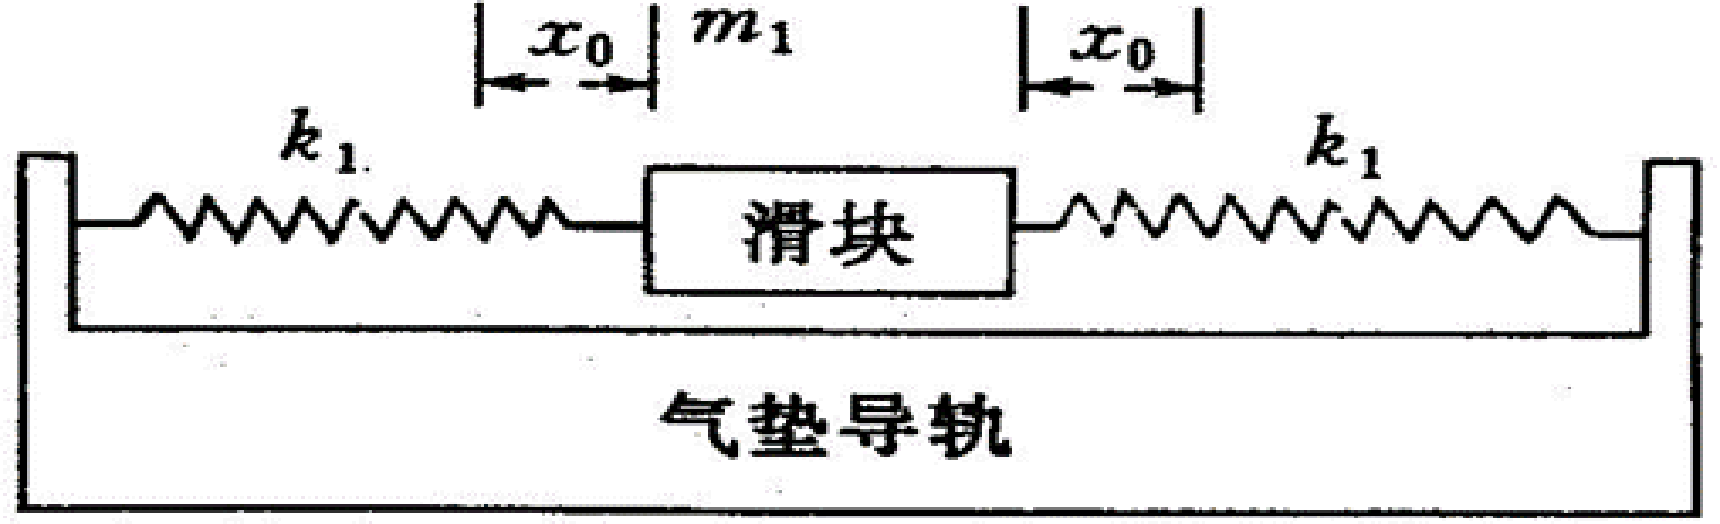
\includegraphics[width=0.6\textwidth]{1.png}
    \caption{\bfseries 弹簧振子示意图}
    \label{fig1}
\end{figure}
由运动方程
\begin{equation}
    -k_{1}(x+x_{0})-[-k_{1}(x-x_{0})]=m\ddot{x}
\end{equation}
令$k=2k_1$\\
方程(1)的解为
\begin{equation}
    x(t)=A\sin(\omega_{0} t+\varphi_{0})
\end{equation}
其中,$A$为振幅,$\omega_{0}=\sqrt{\frac{k}{m}}$为振动系统的固有频率,$\varphi_{0}$为初相位。\\
\begin{equation}
    m=m_{0}+m_{1}
\end{equation}
式中,$m$为振动系统的有效质量;$m_{0}$为弹簧的有效质量;$m_{1}$为滑块和砝码的质量。\\
振动周期$T$与$\omega_{0}$的关系为
\begin{equation}
    T=\frac{2\pi}{\omega_{0}}=2\pi\sqrt{\frac{m}{k}}=2\pi\sqrt{\frac{m_{0}+m_{1}}{k}}
\end{equation}
两边平方即可得到
\begin{equation}
    T^{2}=4\pi^{2}\frac{m_{0}+m_{1}}{k}
\end{equation}
在实验中,我们改变滑块的质量$m_{1}$,测量不同质量下的振动周期$T$,采用作图法获得$T^{2}-m$的图象,通过直线拟合。\\
直线的斜率为
\begin{equation}
    k=\frac{4\pi^{2}}{k}
\end{equation}
同时可以从该条直线的截距获取$m_{0}$。\\








\subsection{简谐运动的运动学特征描述}

对(2)式在时间上进行求导即可得到
\begin{equation}
    v(t)=A\omega_{0}\cos(\omega_{0} t+\varphi_{0})
\end{equation}
由(7)式可见,速度$v$与时间有关,且随时间的变化关系为简谐振动,角频率为$\omega_{0}$,振幅为$A\omega_{0}$,而且速度$v$的相位比$x$超前$\frac{\pi}{2}$\\

综合(2)式和(7)式,消去时间t,可以得到
\begin{equation}
    v^{2}=\omega_{0}^{2}(A^{2}-x^{2})
\end{equation}
即当$x=0$时,速度最大,而当$x=\pm A$时,速度为0。\\










\subsection{简谐振动的机械能}

在实验中,任何时刻系统的振动动能为:
\begin{equation}
    E_{k}=\frac{1}{2}mv^{2}=\frac{1}{2}(m_{0}+m_{1})v^{2}
\end{equation}
系统的弹性势能为(以$m_{1}$位于平衡位置时的系统势能为0)
\begin{equation}
    E_{p}=\frac{1}{2}kx^{2}=\frac{1}{2}kA^{2}\sin^{2}(\omega_{0} t+\varphi_{0})
\end{equation}
系统的机械能为
\begin{equation}
    E=E_{k}+E_{p}=\frac{1}{2}m\omega^{2}A^{2}=\frac{1}{2}kA^{2}
\end{equation}
式中$k$和$A$均不随时间变化。
通过测量滑块$m_1$在不同呢位置$x$的速度$v$,可以计算出系统在不同位置的动能$E_{k}$和势能$E_{p}$,从而验证机械能守恒定律。\\



\subsection{瞬时速度的测定}

在实验中,我们通过测量滑块在不同位置的平均速度,然后通过外推法求出滑块在某一位置的瞬时速度。\\
\begin{equation}
    v=\lim_{\Delta x\rightarrow 0}\frac{\Delta x}{\Delta t}
\end{equation}
我们常用极短时间$\Delta t$内的平均速度$v_{1}$和$v_{2}$的平均值作为瞬时速度$v_{0}$的近似值。\\
\begin{equation}
    \bar{v}=\frac{\Delta s}{\Delta t}
\end{equation}
\begin{figure}[H]
    \centering
    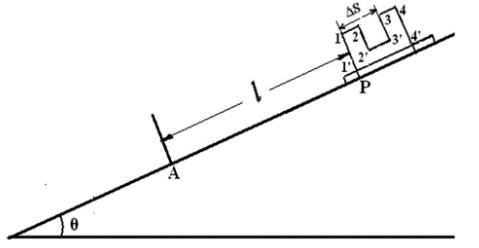
\includegraphics[width=0.6\textwidth]{2.png}
    \caption{\bfseries 测定瞬时速度示意图}
    \label{fig2}
\end{figure}
在实验中,在倾斜的气轨上,于 A 点处放置一光电门,在滑块上先后安装不同挡光距离的 U 型挡光片,使各挡光片的第一挡光边距 A 点为 $l$。滑块每次自 P 点由静止开始下滑,分别测出相应的挡光时间 $\Delta t$ 及挡光距离 $\Delta s$。设滑块由静止下滑距离 $l$ 后的瞬时速度为 $v_0$(即第一挡光时滑块的瞬时速度),则有:
\begin{equation}
\bar{v} = \frac{\Delta s}{\Delta t} = v_0 + \frac{a}{2} \Delta t \quad 
\end{equation}
其中 $a$ 为滑块在 A 附近的加速度。












% ---------------------------------------------------- 

\section{实验内容与步骤}
\subsection{概述}
\begin{enumerate}
    \item 掌握使用光电门测量物体速度和周期的方法。
    \item 验证气垫导轨是否水平,并理解其对实验结果的影响。
    \item 探究弹簧振子的振动周期与振幅、质量的关系。
    \item 分析振动系统的机械能守恒情况。
    \item 研究平均速度与瞬时速度的关系,并使用外推法求瞬时速度。
\end{enumerate}

\subsection{实验步骤}
\begin{enumerate}
    \item \textbf{光电门测速与周期} \\
    使用光电门仪器学习如何测量物体的速度和周期。

    \item \textbf{气垫导轨水平状态验证} \\
    调整气垫导轨至水平状态。通过测量任意两点的速度变化来验证导轨是否真正水平。

    \item \textbf{弹簧振子振动周期与振幅关系} \\
    测量弹簧振子在不同振幅(10.0、20.0、30.0、40.0 cm)下的振动周期。分析实验结果,探讨振幅变化对振动周期的影响。

    \item \textbf{振动周期与振子质量关系} \\
    在滑块上增加不同数量的骑码(铁片),测量增加质量后的振动周期。制作周期平方与质量的图表,并使用最小二乘法进行直线拟合,求出弹簧常数k和滑块质量m0。

    \item \textbf{速度与位移关系} \\
    在滑块上安装U型挡光片,测量不同位移下的速度。制作速度平方与位移平方的图表,并进行直线拟合,验证斜率和截距是否符合理论值。

    \item \textbf{机械能守恒验证} \\
    在固定振幅下,测量滑块在不同位置的速度,并计算动能和势能。比较各位置的机械能,得出能量是否守恒的结论。

    \item \textbf{平均速度与瞬时速度关系} \\
    使用外推法,通过测量不同位移下的平均速度,求出瞬时速度V0。

    \item \textbf{改变气轨倾斜角度} \\
    通过增加垫块数量,改变气轨的倾斜角度θ,并重复上述实验。

    \item \textbf{改变A点到P点的距离} \\
    设置A点到P点的距离为60cm,并重复上述实验。
\end{enumerate}

\subsection{实验结果分析}
对每个实验步骤中得到的数据进行分析和讨论,得出结论,并与理论预期进行对比,验证实验结果的准确性。

\cleardoublepage

\section{实验结果与数据处理}
\subsection{试验仪器的调试}
\begin{table}[H]
    \centering
    \begin{tabular}{|c|c|c|}
        \hline
        V1(cm/s) & V2(cm/s) & 误差\%\\
        \hline
        20.03 & 20.08 & 0.249\\
        \hline
        23.08 & 23.15 & 0.303\\
        \hline
        19.74 & 19.70 & 0.203\\
        \hline
    \end{tabular}
    \caption{\small 实验仪器的调试}
\end{table}
此处皆调至0.5\%以内,可以认为实验仪器调试成功。\\


\subsection{测量弹簧振子的振动周期并考察振动周期和振幅的关系}
\textbf{滑块的振幅A分别取10.0,20.0,30.0,40.0cm时,测量其相应振动周期}
\begin{table}[H]
    \centering
    \begin{tabular}{|c|c|c|c|c|}
        \hline
           & 10cm & 20cm & 30cm & 40cm\\
        \hline
        T1(ms) & 1585.83 & 1585.75 & 1585.81 & 1585.72\\
        \hline
        T2(ms) & 1587.02 & 1585.85 & 1586.04 & 1585.86\\
        \hline
        T3(ms) & 1587.26 & 1585.77 & 1586.17 & 1585.97\\
        \hline
        T4(ms) & 1587.42 & 1585.88 & 1586.05 & 1585.81\\
        \hline
        T5(ms) & 1586.63 & 1586.02 & 1586.02 & 1585.89\\
        \hline
        T(ms) & 1586.832 & 1585.854 & 1585.998 & 1585.85\\
        \hline
    \end{tabular}
    \caption{\small 振动周期与振幅的关系}
\end{table}

\begin{definition}
$T$的值有略微的上升趋势,但是不明显,可以认为振动周期与振幅无关。\\
\indent 若滑块做简谐振动,振动周期与振幅无关,即$T=2\pi\sqrt{\frac{m}{k}}$,$T$与$\sqrt{m}$成正比,而与$A$无关。\\
\end{definition}



\cleardoublepage
\subsection{研究振动周期和振子质量之间的关系}
\textbf{滑块的振幅A取40.0cm,单个骑码质量为25.02g,条型挡光片质量为2.60g}
\begin{table}[H]
    \centering
    \begin{tabular}{|c|c|c|c|c|c|}
        \hline
        滑块个数 & 0 & 1 & 2 & 3 & 4\\
        \hline
        T1(ms) & 1585.65 & 1672.64 & 1755.27 & 1833.59 & 1909.09\\
        \hline
        T2(ms) & 1585.87 & 1672.83 & 1755.23 & 1833.45 & 1909.64\\
        \hline
        T3(ms) & 1585.93 & 1672.74 & 1755.19 & 1833.56 & 1909.48\\
        \hline
        T4(ms) & 1586.00 & 1672.83 & 1755.24 & 1833.55 & 1909.24\\
        \hline
        T5(ms) & 1586.05 & 1672.68 & 1755.27 & 1833.83 & 1909.66\\
        \hline
        T6(ms) & 1586.08 & 1672.65 & 1755.25 & 1834.03 & 1909.88\\
        \hline
        T7(ms) & 1586.10 & 1672.59 & 1755.34 & 1833.95 & 1909.84\\
        \hline
        T8(ms) & 1586.03 & 1672.51 & 1755.28 & 1834.01 & 1909.70\\
        \hline
        T9(ms) & 1586.21 & 1672.65 & 1755.25 & 1834.15 & 1909.16\\
        \hline
        T10(ms) & 1586.19 & 1672.42 & 1755.12 & 1833.81 & 1909.51\\
        \hline
        \textbf{T(ms)} & 1586.011 & 1672.654 & 1755.244 & 1833.753 & 1909.52\\
        \hline			
    \end{tabular}
    \caption{\small 振动周期与振子质量关系}
\end{table}

滑块质量$213.03g$,条形挡光片质量$2.60g$,骑码质量$25.02g$\\
\indent 进行最小二乘法拟合,且直线方程为$T^{2}=4\pi^{2}\frac{m_{0}+m_{1}}{k}$\\

\begin{figure}[H]
    \centering
    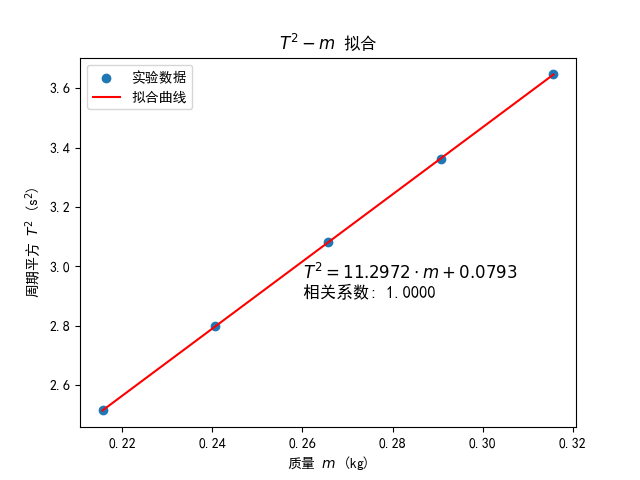
\includegraphics[width=0.9\textwidth]{Figure_1.png}
    \caption{\bfseries 振动周期与振子质量关系最小二乘法}
    \label{$T^2-m最小二乘法拟合图像$}
\end{figure}

\indent 通过Theil-Sen估计法,且直线方程为$T^{2}=4\pi^{2}\frac{m_{0}+m_{1}}{k}$\\

\begin{figure}[H]
    \centering
    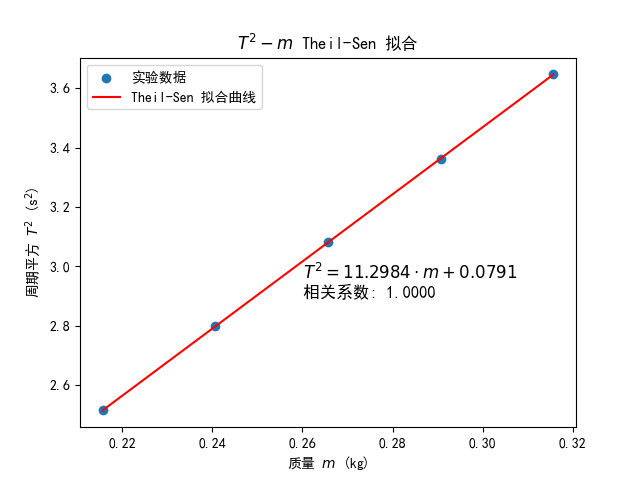
\includegraphics[width=0.9\textwidth]{Figure_2.png}
    \caption{\bfseries 振动周期与振子质量关系Theil-Sen估计法}
    \label{$T^2-m Theil-Sen估计拟合图像$}
\end{figure}

\indent 这里老师要求用两种不同的方法进行拟合,可以看到两种方法得到的结果略有差异,且相关系数都是非常接近1,说明拟合的效果较好。\\

\indent 根据公式得到直线斜率为$\frac{4\pi^2}{k}$,截距为$\frac{4\pi^2m_0}{k}$\\

\indent 通过最小二乘法得到的斜率为$11.2972$,截距为$0.0793$\\

\indent 代入数据得到$k=3.494N/m$, $m_0=7.01944g$\\

\indent 通过Theil-Sen估计法得到的斜率为$11.2984$,截距为$0.0791$\\

\indent 代入数据得到$k=3.493N/m$, $m_0=7.00099g$\\


\cleardoublepage
\subsection{研究速度与位移之间的关系}
\textbf{滑块的振幅A取40.0cm}

\begin{table}[H]
    \centering
    \begin{tabular}{|c|c|c|c|c|c|}
        \hline
        x(cm) & 10 & 15 & 20 & 25 & 30\\
        \hline
        V1(cm/s) & 144.51 & 138.70 & 131.23 & 117.37 & 100.40\\
        \hline
        V2(cm/s) & 143.47 & 136.61 & 129.87 & 115.61 & 98.33\\
        \hline
        V3(cm/s) & 141.04 & 135.52 & 127.55 & 113.25 & 95.24\\
        \hline
        \textbf{V(cm/s)} & \textbf{143.01} & \textbf{136.28} & \textbf{129.55} & \textbf{115.41} & \textbf{97.99}\\
        \hline			
    \end{tabular}
    \caption{\small 速度与位移关系}
\end{table}

\begin{figure}[H]
    \centering
    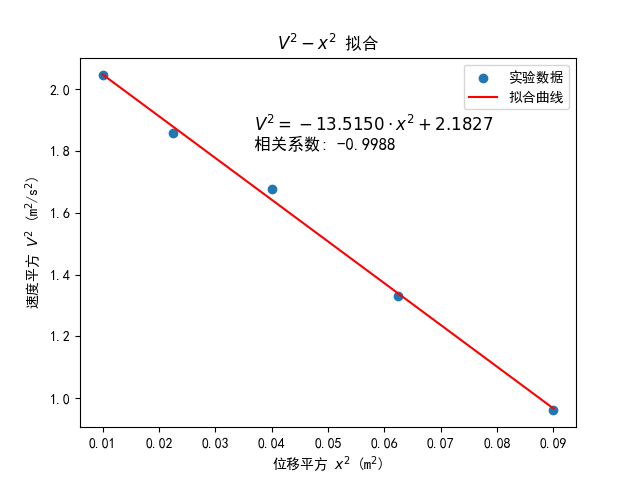
\includegraphics[width=0.9\textwidth]{Figure_3.png}
    \caption{\bfseries 速度与位移关系}
    \label{速度与位移关系}
\end{figure}

\indent 由实验第三步中得到$T=1.586s$,$\omega_0=\frac{2\pi}{T}=3.962s^{-1}$

\indent 由斜率$k=-13.5150$,截距$b=2.1827$

\indent 而$-\omega_0^2=-15.695$,$A^2\omega_0^2=2.5112$

\indent 由此可以看出,实验数据与理论值有一定的偏差,可能的原因有。\\

\begin{enumerate}
    \item 测量误差
        \begin{itemize}
            \item 光电门精度:如果使用光电门来测量滑块的速度,光电门的响应时间或灵敏度可能会导致测量不准确。特别是在滑块快速运动时,光电门可能未能准确捕捉滑块的通过时间,导致速度数据不精确。
            \item 位置测量误差:位移的测量通常通过标尺、光电门或编码器等设备进行,如果这些设备的精度不高或安装不稳固,测得的位移数据可能会出现偏差。
        \end{itemize}
    \item 时间延迟和同步误差
        \begin{itemize}
            \item 在测量过程中,光电门、传感器和记录设备之间的时间延迟可能导致同步误差。如果位移和速度的测量没有精确同步(例如,光电门的触发时间和数据采集时间之间的延迟),就可能导致速度和位移之间的关系出现偏差。
        \end{itemize}
    \item 阻尼效应
        \begin{itemize}
            \item 在实际实验中,阻尼(如空气阻力或摩擦力)会使滑块的振动逐渐减弱。阻尼效应使得速度和位移的关系不再完全符合理想的公式(如 $v = \frac{dx}{dt}$)。这可能导致速度和位移之间的关系逐渐偏离理想简谐振动的理论模型。
        \end{itemize}
\end{enumerate}


\subsection{研究振动系统的机械能是否守恒}
\textbf{滑块的振幅A取40.0cm}

\begin{table}[H]
    \centering
    \begin{tabular}{|c|c|c|c|c|c|}
        \hline
        x(cm) & 10 & 15 & 20 & 25 & 30\\
        \hline
        V(cm/s) & 143.01 & 136.28 & 129.55 & 115.41 & 97.99\\
        \hline
        $E_k$(J) & 0.2205 & 0.2002 & 0.1809 & 0.1436 & 0.1035\\
        \hline
        $E_p$(J) & 0.01747 & 0.03931 & 0.06988 & 0.10919 & 0.15723\\
        \hline
        E(J) & 0.23797 & 0.23951 & 0.25078 & 0.25279 & 0.26073\\
        \hline			
    \end{tabular}
    \caption{\small 机械能守恒}
\end{table}

由实验4中得到$k=3.494N/m$, $m=215.63g$\\
\[
E_k=\frac{1}{2}m_0v^2, E_p=\frac{1}{2}kx^2
\]
\[
E=E_k+E_p
\]
\indent 计算得到的机械能均值为$0.24856J$\\
\indent 最大误差为$0.01217J$,约为$4.896\%$\\
\indent 由此可以看出,实验数据与理论值有一定的偏差,可能的原因有:
\begin{enumerate}
    \item 势能测量较为准确,而动能测量存在一定误差。
    \item 光电门的响应时间:光电门或其他传感器可能存在响应延迟。在高速运动时,滑块通过光电门的时间变得非常短,如果光电门的响应时间较长,可能会无法精确捕捉滑块的瞬时位置和速度,导致测量出的速度偏小。
\end{enumerate}


\subsection{改变弹簧振子的振幅$A$,测相应的$V_{max}$,由$V_{max}^2$与$A^2$的关系求出$k$,与实验内容3的结果进行比较}

\begin{table}[H]
    \centering
    \begin{tabular}{|c|c|c|c|c|c|}
        \hline
         & 10cm & 15cm & 20cm & 25cm & 30cm\\
        \hline
        $V_{max1}$(cm/s) & 40.62 & 56.85 & 75.87 & 95.42 & 116.41\\
        \hline
        $V_{max2}$(cm/s) & 39.82 & 55.96 & 74.92 & 94.34 & 114.81\\
        \hline
        $V_{max3}$(cm/s) & 39.12 & 55.28 & 74.10 & 93.37 & 113.76\\
        \hline
        \textbf{$V_{max}$(cm/s)} & \textbf{39.85} & \textbf{56.03} & \textbf{74.96} & \textbf{94.38} & \textbf{114.99}\\
        \hline			
    \end{tabular}
    \caption{\small $V_{max}^2$与$A^2$的关系}
\end{table}

\begin{figure}[H]
    \centering
    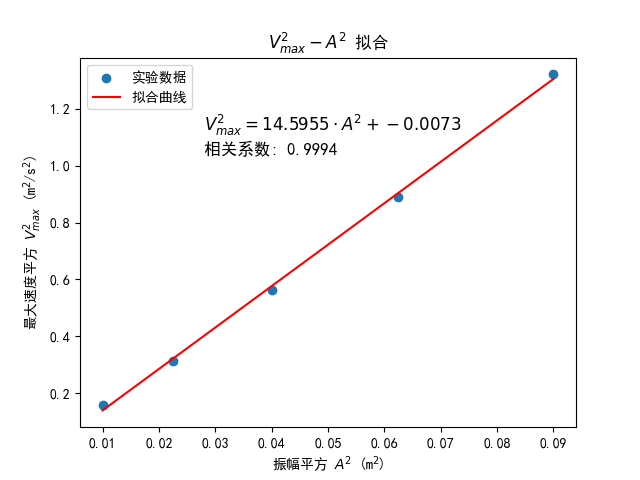
\includegraphics[width=0.9\textwidth]{Figure_4.png}
    \caption{\bfseries $V_{max}^2$与$A^2$的关系}
\end{figure}

\begin{enumerate}
    \item 拟合效果较好,相关系数接近 1,斜率为 $14.5955$,截距为 $-0.0073$。
    \item 又 $m_0 = 7.01944 \, \text{g}$,$m_1 = 215.63 \, \text{g}$。
    \item 由 $V_{max}^2$ 和 $A^2$ 的关系知,$k = (m_0 + m_1) \times 14.5955 = 3.250 \, \text{N/m}$。
    \item 和实验 3 中的结果进行比较,可以看出两种方法得到的结果略有差异,误差约为 $7.1\%$。
    \item 可能的原因有:测量误差、实验环境的影响、数据处理方法的不同等。以及上面提到的光电门或其他传感器可能存在响应延迟。在高速运动时,滑块通过光电门的时间变得非常短,如果光电门的响应时间较长,可能会无法精确捕捉滑块的瞬时位置和速度,导致测量出的速度偏小。
\end{enumerate}


\subsection{实验中可能用到的其他相关参数}
滑块的质量$m=25.02g$,条型挡光片的质量$m=2.60g$,U型挡光片的质量$m=11.86g$


\subsection{测定瞬时速度,测量不同U挡光片通过光电门所用的时间(AP距离为50cm),计算平均速度。}

\begin{table}[H]
    \centering
    \begin{tabular}{|c|c|c|c|c|c|c|c|}
        \hline
        挡光片宽度(cm) & $\Delta t_1$(ms) & $\Delta t_2$(ms) & $\Delta t_3$(ms) & $\Delta t_4$(ms) & $\Delta t_5$(ms) & $\Delta t$(ms) & v(m/s)\\
        \hline
        1(cm) & 30.88 & 30.46 & 30.59 & 30.66 & 30.61 & \textbf{30.64} & \textbf{0.3264}\\
        \hline
        3(cm) & 93.11 & 90.98 & 92.75 & 92.68 & 92.26 & \textbf{92.36} & \textbf{0.3248}\\
        \hline
        5(cm) & 153.55 & 152.64 & 153.97 & 155.16 & 154.21 & \textbf{153.91} & \textbf{0.3249}\\
        \hline
        10(cm) & 294.00 & 294.13 & 288.60 & 288.81 & 290.55 & \textbf{291.22} & \textbf{0.3434}\\
        \hline		
    \end{tabular}
    \caption{\small 测定瞬时速度}
\end{table}

\begin{figure}[H]
    \centering
    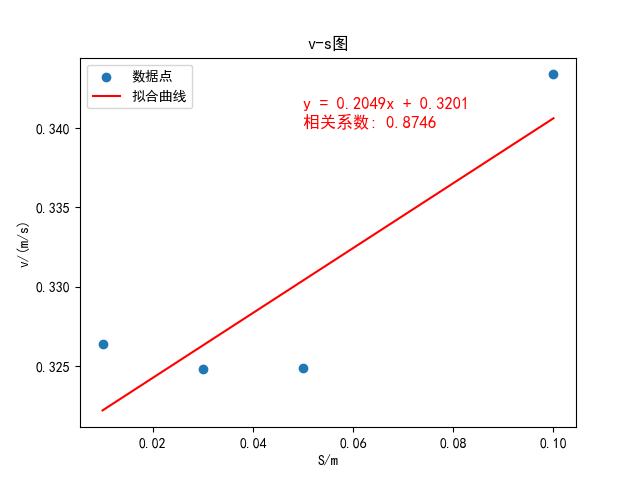
\includegraphics[width=0.9\textwidth]{Figure_5.png}
    \caption{\bfseries v-s关系}
\end{figure}

\begin{figure}[H]
    \centering
    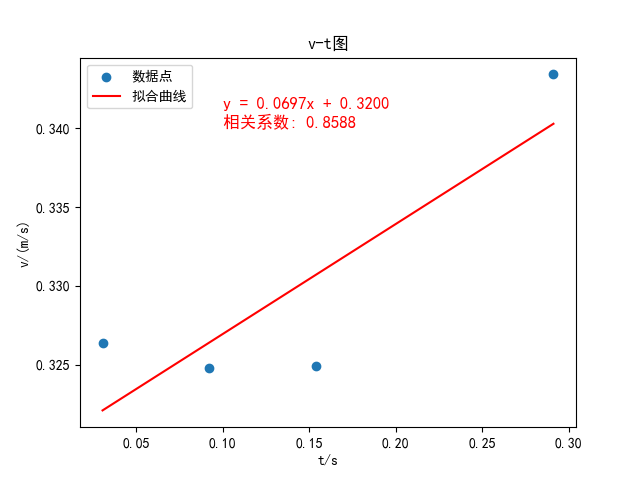
\includegraphics[width=0.9\textwidth]{Figure_6.png}
    \caption{\bfseries v-t关系}
\end{figure}

\indent 由上面两张拟合图像的截距分别为0.3201和0.3200,非常接近,故可以认为通过光电门的瞬时速度为0.32005m/s。\\


\subsection{测定瞬时速度,改变导轨倾斜角度,测量不同U挡光片通过光电门所用的时间(AP)距离为50(cm),计算平均速度。}

\begin{table}[H]
    \centering
    \begin{tabular}{|c|c|c|c|c|c|c|c|}
        \hline
        挡光片宽度(cm) & $\Delta t_1$(ms) & $\Delta t_2$(ms) & $\Delta t_3$(ms) & $\Delta t_4$(ms) & $\Delta t_5$(ms) & $\Delta t$(ms) & v(m/s)\\
        \hline
        1(cm) & 21.67 & 21.32 & 21.44 & 21.63 & 21.32 & \textbf{21.48} & \textbf{0.4655}\\
        \hline
        3(cm) & 63.86 & 64.32 & 63.76 & 63.94 & 64.11 & \textbf{64.00} & \textbf{0.4688}\\
        \hline
        5(cm) & 104.89 & 105.65 & 104.69 & 104.93 & 105.02 & \textbf{105.04} & \textbf{0.4760}\\
        \hline
        10(cm) & 204.83 & 206.53 & 206.69 & 206.33 & 205.78 & \textbf{206.03} & \textbf{0.4854}\\
        \hline		
    \end{tabular}
    \caption{\small 测定瞬时速度,改变导轨倾斜角度}
\end{table}


\begin{figure}[H]
    \centering
    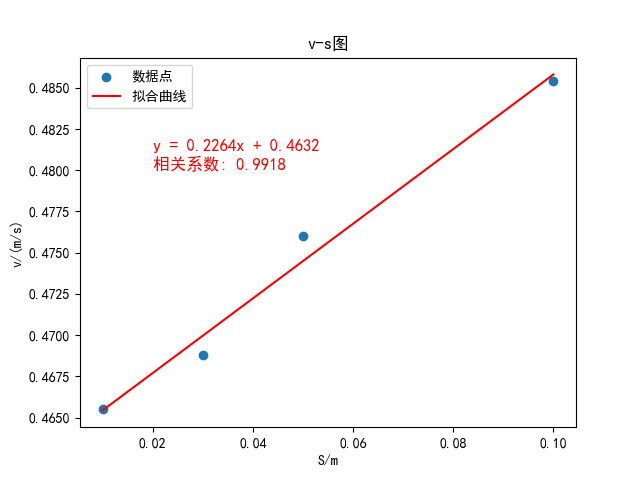
\includegraphics[width=0.9\textwidth]{Figure_7.png}
    \caption{\bfseries v-s关系}
\end{figure}

\begin{figure}[H]
    \centering
    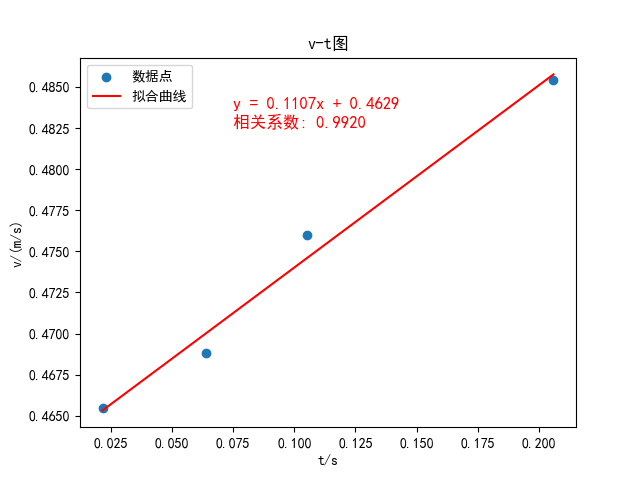
\includegraphics[width=0.9\textwidth]{Figure_8.png}
    \caption{\bfseries v-t关系}
\end{figure}

\indent 由上面两张拟合图像的截距分别为0.4632和0.4629,非常接近,故可以认为通过光电门的瞬时速度为0.46305m/s。\\






\subsection{测定瞬时速度,改变AP距离为60(cm),测量不同U挡光片通过光电门所用的时间,计算平均速度。}

\begin{table}[H]
    \centering
    \begin{tabular}{|c|c|c|c|c|c|c|c|}
        \hline
        挡光片宽度(cm) & $\Delta t_1$(ms) & $\Delta t_2$(ms) & $\Delta t_3$(ms) & $\Delta t_4$(ms) & $\Delta t_5$(ms) & $\Delta t$(ms) & v(m/s)\\
        \hline
        1(cm) & 27.73 & 27.90 & 27.65 & 27.87 & 27.80 & \textbf{27.79} & \textbf{0.3598}\\
        \hline
        3(cm) & 81.90 & 82.74 & 82.35 & 83.02 & 82.27 & \textbf{82.46} & \textbf{0.3638}\\
        \hline
        5(cm) & 136.58 & 135.35 & 135.28 & 136.40 & 135.43 & \textbf{135.81} & \textbf{0.3682}\\
        \hline
        10(cm) & 264.82 & 265.64 & 268.53 & 266.39 & 265.73 & \textbf{266.22} & \textbf{0.3756}\\
        \hline			
    \end{tabular}
    \caption{\small 测定瞬时速度,改变AP距离为60(cm)}
\end{table}


\begin{figure}[H]
    \centering
    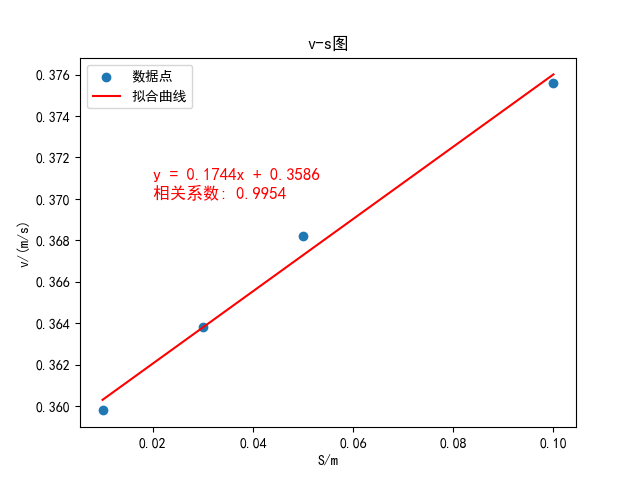
\includegraphics[width=0.9\textwidth]{Figure_9.png}
    \caption{\bfseries v-s关系}
\end{figure}

\begin{figure}[H]
    \centering
    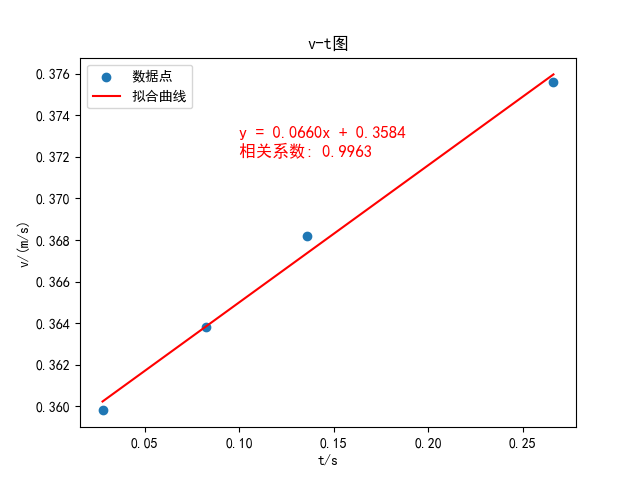
\includegraphics[width=0.9\textwidth]{Figure_10.png}
    \caption{\bfseries v-t关系}
\end{figure}

\indent 由上面两张拟合图像的截距分别为0.3586和0.3584,非常接近,故可以认为通过光电门的瞬时速度为0.3585m/s。\\


\subsection{附加实验:落球法测定液体(蓖麻油)在不同温度的粘度}
\textbf{测定液体(蓖麻油)在30$^{\circ}C$时的粘度}\\
小球的尺寸$d=1.20\pm 0.02mm$,密度$\rho =7.8\times 10^3 kg/m^3$,液体(蓖麻油)密度$\rho_0 = 0.95\times 10^3 kg/m^3$,管直径$D=2.6\times 10^{-2}m$,小球运动的距离$L=0.2m$\\
\begin{table}[H]
    \begin{table}[H]
        \centering
        \begin{tabular}{|c|c|c|c|c|c|c|c|c|}
            \hline
            \diagbox{温度($^{\circ}C$)}{测量次数} & 1 & 2 & 3 & 4 & 平均时间(s) & 测得$\eta (Pa\cdot s)$ & 标准$\eta (Pa\cdot s)$\\
            \hline
            30$^{\circ}C$ & 18.50s & 18.19s & 18.40s & 18.32s & 18.3525s & 0.444 & 0.451\\
            \hline			
        \end{tabular}
        \caption{\small 落球法测定液体(蓖麻油)粘度}
    \end{table}
\end{table}

由公式
\[
\eta = \frac{(\rho - \rho_0)gd^2}{18v_0(1+2.4d/D)}
\]
其中
\[
v_0 = \frac{L}{t}=0.2/18.3525=0.0109m/s
\]
\[
\eta = \frac{(7.8\times 10^3-0.95\times 10^3)\times 9.8m/s^2\times 1.20^2\times 10^{-6}}{18\times 0.0109(1+2.4\times 1.20/26)}=0.444Pa\cdot s
\]
实验误差约为$1.65\%$\\
该实验的误差主要来源于以下几个方面:
\begin{enumerate}
    \item 小球的尺寸测量误差:小球的尺寸测量可能存在一定的误差,导致计算液体粘度时的数据不准确。
    \item 测量时间误差:测量小球下落时间时,计时器的精度和人为操作的误差可能会导致测量时间的误差。
\end{enumerate}





\section{实验总结}

\subsection{讲义思考题}

\begin{enumerate}
    \item \textbf{为什么滑块可以认为是做简谐振动?实验中如何保证滑块做简谐振动?}
    
    滑块的振幅减小是因为存在阻尼,但在气垫导轨的设计下,摩擦阻力被尽可能减小,阻尼效应相对较小,因此在不考虑能量耗散的情况下,可以近似认为滑块做简谐振动。为了保证实验中滑块尽量做简谐振动,应该确保气垫导轨保持水平,减少空气阻力和摩擦力的影响,并使用光电门等精确测量工具来记录滑块的振动数据。

    \item \textbf{弹簧的等效质量的物理意义,如不考虑弹簧的等效质量,对实验结果有何影响?}
    
    弹簧的等效质量指的是弹簧本身的质量对系统运动的影响。在振动实验中,弹簧的质量会引起系统的固有频率变化,忽略这一因素会导致实验结果出现偏差。具体来说,如果不考虑弹簧的等效质量,系统的总质量 \(m\) 将被低估,这会导致实验中动能偏小,进而导致机械能的偏小计算。在使用 \(k\) 的值时,也会因未考虑弹簧的质量而导致偏小,从而影响实验中机械能守恒定律的验证。

    \item \textbf{测量周期时,光电门是否必须在平衡位置上?如果不在平衡位置会产生什么不同的效果?}
    
    光电门不一定必须放在平衡位置,只要它位于振动范围内即可。因为周期性是由振动的全程控制的,在一个完整的周期内,任何位置的测量时间都应该是相等的。但若光电门不在平衡位置,可能会因为阻尼效应而导致周期的测量误差,因为滑块每次通过光电门时,可能处于不同的振动相位,从而影响周期的精确测量。

    \item \textbf{气垫导轨如果不水平,是否能进行该实验?}
    
    如果气垫导轨不水平,会导致滑块的运动受到重力的额外影响,产生额外的势能变化,这会影响实验数据的准确性。特别是在验证机械能守恒时,若气垫导轨不水平,无法精确测量重力势能变化,进而不能进行精确的机械能守恒实验。因此,气垫导轨必须水平才能保证实验的准确性。

    \item \textbf{使用平板型挡光片和两个光电门,如何测量滑块通过倾斜气轨上某一点的瞬时速度?}
    
    在测量滑块通过倾斜气轨某一点的瞬时速度时,可以将两个光电门设置在该点的左右对称位置,确保它们之间的距离非常小。通过测量滑块从一个光电门到另一个光电门的时间差,再根据光电门之间的已知距离,就可以计算出滑块的瞬时速度。需要保证光电门与气轨的角度一致,以避免因角度差异带来的测量误差。

    \item \textbf{气垫导轨如果不水平,对瞬时速度的测定有什么影响?}
    
    如果气垫导轨不水平,滑块将受到非水平重力分力的影响,导致滑块的加速度发生变化。虽然瞬时速度的测定主要依赖于光电门测量时间和距离,但气垫导轨的不水平性可能会引入偏差,导致计算出的瞬时速度存在误差,尤其是在斜面角度较大的情况下,误差会更加明显。

    \item \textbf{每次测量滑块和 U 型挡光片的总质量不同,是否对瞬时速度的测定有影响?}
    
    对于滑块和 U 型挡光片的总质量的变化,它不会影响瞬时速度的测定,因为在倾斜气轨上,滑块和挡光片的质量变化不会改变重力加速度的分量。重力加速度与质量成正比,但在计算过程中质量会被消去。因此,质量变化不会对瞬时速度的测定产生影响。
\end{enumerate}

\subsection{实验中的问题与感想}

\begin{enumerate}
    \item 在实验过程中,由于气垫导轨的水平度对实验结果有很大的影响,因此在实验前要对气垫导轨进行调整,保证其水平度。祝老师要求需要三次调至误差在 0.3\% 下方能继续实验。

    \item 在我调水平的时候,发现了空气阻力对于滑块速度也存在影响。在较低速的时候,误差值在 1\%-2\% 之间,而在较高速的时候,误差值在 0.2\%-0.3\% 之间。这说明空气阻力对于滑块速度的影响是非常大的。
    
    \item 在实验过程中会使用到挡光片,在调整的时候也要注意挡光片不会与光电门发生摩擦,否则会影响实验结果。
    
    \item 实验过程中,数字毫秒计在使用时可能会出现问题,我在使用过程中发现数据会突然变得很大或者稳定在 1 左右,这个时候需要换一下光电门的接口或者重启一下数字毫秒计。
    
    \item 在最后三个实验中,我们要注意滑块下滑的位置,U 型挡光片前侧挡光片需要与在平衡位置的光电门间隔所要求的距离,而不是两个挡光片中间的位置,尤其是挡光片尺寸越大操作失误导致的误差也会更大。
    
    \item 课堂上要积极回答问题,这样可以更好地锻炼自己的思维能力,也可以更好地理解实验的原理。(课堂上回答了两个问题让我对实验细节的认识更加清晰)
    
    \item 老师对实验原理和过程的细致讲解让我在预习的基础上对实验有了更深的认识,实验过程中数字毫秒计的问题也得到了老师的帮助而解决,非常感谢老师的耐心。
    
    \item 最后需要提到的是,在撰写实验报告的时候,我发现我没有将测量的滑块的质量记录下来,而当时祝老师还单独提醒我记录数据,导致在实验第二天下午我还去了实验室重新测量了一次滑块的质量,这也提醒我在实验过程中要注意记录数据。
\end{enumerate}


\cleardoublepage
\section{附录:拟合用Python 代码}

\begin{lstlisting}[language=Python, caption=Figure's Python code, label=code:python_example]
#Figure_1.py
    import numpy as np
import matplotlib.pyplot as plt
from matplotlib import rcParams

# 设置中文字体
rcParams['font.sans-serif'] = ['SimHei']  # 使用黑体
rcParams['axes.unicode_minus'] = False  # 解决负号显示问题

# 数据
n = np.array([0, 1, 2, 3, 4])
T_ms = np.array([1586.011, 1672.654, 1755.244, 1833.753, 1909.52])
T_s = T_ms / 1000  # 将时间单位从毫秒转换为秒
m1 = (213.03+2.60) / 1000  # 滑块加条形挡光片质量,单位为kg
m2 = 25.02 / 1000    # 骑码质量,单位为kg
m = m1 + n * m2  # 总质量,单位为kg

# 进行线性拟合
coefficients = np.polyfit(m, T_s**2, 1)
poly = np.poly1d(coefficients)

# 计算相关系数
correlation_matrix = np.corrcoef(m, T_s**2)
correlation_coefficient = correlation_matrix[0, 1]

# 拟合结果
print(f"拟合得到的系数: {coefficients}")
print(f"相关系数: {correlation_coefficient}")

# 绘图
plt.scatter(m, T_s**2, label='实验数据')
plt.plot(m, poly(m), label='拟合曲线', color='red')

# 显示图线方程和相关系数
equation_text = f'$T^2 = {coefficients[0]:.4f} \cdot m + {coefficients[1]:.4f}$\n相关系数: {correlation_coefficient:.4f}'
plt.text(0.45, 0.45, equation_text, transform=plt.gca().transAxes, fontsize=12, verticalalignment='top')

plt.xlabel('质量 $m$ (kg)')
plt.ylabel('周期平方 $T^2$ (s$^2$)')
plt.legend()
plt.title('$T^2 - m$ 拟合')
plt.show()






#Figure_2.py
import numpy as np
import matplotlib.pyplot as plt
from sklearn.linear_model import TheilSenRegressor
from matplotlib import rcParams

# 设置中文字体
rcParams['font.sans-serif'] = ['SimHei']  # 使用黑体
rcParams['axes.unicode_minus'] = False  # 解决负号显示问题

# 数据
n = np.array([0, 1, 2, 3, 4])
T_ms = np.array([1586.011, 1672.654, 1755.244, 1833.753, 1909.52])
T_s = T_ms / 1000  # 将时间单位从毫秒转换为秒
m1 = (213.03+2.60) / 1000  # 滑块加条形挡光片质量,单位为kg
m2 = 25.02 / 1000    # 骑码质量,单位为kg
m = m1 + n * m2  # 总质量,单位为kg

# 进行 Theil-Sen 估计线性拟合
model = TheilSenRegressor()
m_reshaped = m.reshape(-1, 1)  # 将 m 转换为二维数组
model.fit(m_reshaped, T_s**2)
a = model.coef_[0]
b = model.intercept_

# 计算相关系数
correlation_matrix = np.corrcoef(m, T_s**2)
correlation_coefficient = correlation_matrix[0, 1]

# 拟合结果
print(f"拟合得到的系数: a = {a}, b = {b}")
print(f"相关系数: {correlation_coefficient}")

# 绘图
plt.scatter(m, T_s**2, label='实验数据')
plt.plot(m, model.predict(m_reshaped), label='Theil-Sen 拟合曲线', color='red')

# 显示图线方程和相关系数
equation_text = f'$T^2 = {a:.4f} \cdot m + {b:.4f}$\n相关系数: {correlation_coefficient:.4f}'
plt.text(0.45, 0.45, equation_text, transform=plt.gca().transAxes, fontsize=12, verticalalignment='top')

plt.xlabel('质量 $m$ (kg)')
plt.ylabel('周期平方 $T^2$ (s$^2$)')
plt.legend()
plt.title('$T^2 - m$ Theil-Sen 拟合')
plt.show()




#Figure_3.py
import numpy as np
import matplotlib.pyplot as plt
from matplotlib import rcParams

# 设置中文字体
rcParams['font.sans-serif'] = ['SimHei']  # 使用黑体
rcParams['axes.unicode_minus'] = False  # 解决负号显示问题

# 数据
V = np.array([143.01, 136.28, 129.55, 115.41, 97.99]) / 100  # 将速度除以100
x = np.array([10, 15, 20, 25, 30]) / 100  # 将位移除以100

# 转化为平方
V_squared = V**2
x_squared = x**2

# 进行线性拟合
coefficients = np.polyfit(x_squared, V_squared, 1)
poly = np.poly1d(coefficients)

# 计算相关系数
correlation_matrix = np.corrcoef(x_squared, V_squared)
correlation_coefficient = correlation_matrix[0, 1]

# 拟合结果
print(f"拟合得到的系数: {coefficients}")
print(f"相关系数: {correlation_coefficient}")

# 绘图
plt.scatter(x_squared, V_squared, label='实验数据')
plt.plot(x_squared, poly(x_squared), label='拟合曲线', color='red')

# 显示图线方程和相关系数
equation_text = f'$V^2 = {coefficients[0]:.4f} \cdot x^2 + {coefficients[1]:.4f}$\n相关系数: {correlation_coefficient:.4f}'
plt.text(0.35, 0.85, equation_text, transform=plt.gca().transAxes, fontsize=12, verticalalignment='top')

plt.xlabel('位移平方 $x^2$ (m$^2$)')
plt.ylabel('速度平方 $V^2$ (m$^2$/s$^2$)')
plt.legend()
plt.title('$V^2 - x^2$ 拟合')
plt.show()








#Figure_4.py
import numpy as np
import matplotlib.pyplot as plt
from matplotlib import rcParams

# 设置中文字体
rcParams['font.sans-serif'] = ['SimHei']  # 使用黑体
rcParams['axes.unicode_minus'] = False  # 解决负号显示问题

# 数据
A = np.array([10, 15, 20, 25, 30]) / 100  # 将振幅除以100
V_max = np.array([39.85, 56.03, 74.96, 94.38, 114.99]) / 100  # 将最大速度除以100

# 转化为平方
A_squared = A**2
V_max_squared = V_max**2

# 进行线性拟合
coefficients = np.polyfit(A_squared, V_max_squared, 1)
poly = np.poly1d(coefficients)

# 计算相关系数
correlation_matrix = np.corrcoef(A_squared, V_max_squared)
correlation_coefficient = correlation_matrix[0, 1]

# 拟合结果
print(f"拟合得到的系数: {coefficients}")
print(f"相关系数: {correlation_coefficient}")

# 绘图
plt.scatter(A_squared, V_max_squared, label='实验数据')
plt.plot(A_squared, poly(A_squared), label='拟合曲线', color='red')

# 显示图线方程和相关系数
equation_text = f'$V_{{max}}^2 = {coefficients[0]:.4f} \cdot A^2 + {coefficients[1]:.4f}$\n相关系数: {correlation_coefficient:.4f}'
plt.text(0.25, 0.85, equation_text, transform=plt.gca().transAxes, fontsize=12, verticalalignment='top')

plt.xlabel('振幅平方 $A^2$ (m$^2$)')
plt.ylabel('最大速度平方 $V_{max}^2$ (m$^2$/s$^2$)')
plt.legend()
plt.title('$V_{max}^2 - A^2$ 拟合')
plt.show()








#Figure_5.py
import numpy as np
import matplotlib.pyplot as plt
from matplotlib import rcParams

# 设置中文字体
rcParams['font.sans-serif'] = ['SimHei']  # 使用黑体
rcParams['axes.unicode_minus'] = False  # 解决负号显示问题

# 数据点
s_data = np.array([1, 3, 5, 10])/100
v_data = np.array([0.3264, 0.3248, 0.3249, 0.3434])

# 进行线性拟合
coefficients = np.polyfit(s_data, v_data, 1)
a, b = coefficients

# 生成拟合直线的y值
v_fit = np.polyval(coefficients, s_data)

# 计算相关系数
correlation_matrix = np.corrcoef(s_data, v_data)
correlation_coefficient = correlation_matrix[0, 1]

# 绘制数据点和拟合曲线
plt.scatter(s_data, v_data, label='数据点')
plt.plot(s_data, v_fit, color='red', label='拟合曲线')

# 添加拟合直线方程和相关系数
equation_text = f'y = {a:.4f}x + {b:.4f}\n相关系数: {correlation_coefficient:.4f}'
plt.text(0.05, 0.34, equation_text, fontsize=12, color='red')

# 添加图表标题
plt.title('v-s图')

plt.xlabel('S/m')
plt.ylabel('v/(m/s)')
plt.legend()
plt.show()













#Figure_6.py
import numpy as np
import matplotlib.pyplot as plt
from matplotlib import rcParams

# 设置中文字体
rcParams['font.sans-serif'] = ['SimHei']  # 使用黑体
rcParams['axes.unicode_minus'] = False  # 解决负号显示问题

# 数据点
t_data = np.array([30.64, 92.36, 153.91, 291.22])/1000
v_data = np.array([0.3264, 0.3248, 0.3249, 0.3434])

# 进行线性拟合
coefficients = np.polyfit(t_data, v_data, 1)
a, b = coefficients

# 生成拟合直线的y值
v_fit = np.polyval(coefficients, t_data)

# 计算相关系数
correlation_matrix = np.corrcoef(t_data, v_data)
correlation_coefficient = correlation_matrix[0, 1]

# 绘制数据点和拟合曲线
plt.scatter(t_data, v_data, label='数据点')
plt.plot(t_data, v_fit, color='red', label='拟合曲线')

# 添加拟合直线方程和相关系数
equation_text = f'y = {a:.4f}x + {b:.4f}\n相关系数: {correlation_coefficient:.4f}'
plt.text(0.10, 0.34, equation_text, fontsize=12, color='red')

# 添加图表标题
plt.title('v-t图')

plt.xlabel('t/s')
plt.ylabel('v/(m/s)')
plt.legend()
plt.show()

###Figure_7,8,9,10.py 代码与Figure_5.py和Figure_6.py类似,不再赘述
\end{lstlisting}



\section{实验原始数据表}

\begin{figure}[H]
    \centering
    \includegraphics[width=0.9\textwidth]{sy1.jpg}
    \caption{\bfseries 实验数据表}
\end{figure}

\begin{figure}[H]
    \centering
    \includegraphics[width=0.9\textwidth]{sy2.jpg}
    \caption{\bfseries 实验数据表}
\end{figure}

\begin{figure}[H]
    \centering
    \includegraphics[width=0.9\textwidth]{sy3.jpg}
    \caption{\bfseries 实验数据表}
\end{figure}

\end{document}

% VScode 常用快捷键:

% F2:                       变量重命名
% Ctrl + Enter:             行中换行
% Alt + up/down:            上下移行
% 鼠标中键 + 移动:           快速多光标
% Shift + Alt + up/down:    上下复制
% Ctrl + left/right:        左右跳单词
% Ctrl + Backspace/Delete:  左右删单词    
% Shift + Delete:           删除此行
% Ctrl + J:                 打开 VScode 下栏(输出栏)
% Ctrl + B:                 打开 VScode 左栏(目录栏)
% Ctrl + `:                 打开 VScode 终端栏
% Ctrl + 0:                 定位文件
% Ctrl + Tab:               切换已打开的文件(切标签)
% Ctrl + Shift + P:         打开全局命令(设置)

% Latex 常用快捷键:

% Ctrl + Alt + J:           由代码定位到PDF
% Ctrl + S:                 保存